\documentclass{beamer}
\usepackage{amsfonts,amsmath,oldgerm}
\usetheme{sintef}
\usepackage{listings}
\usepackage{xcolor}
\usepackage{amsmath}
\usepackage{tikz}
\usepackage{graphicx}
\definecolor{codegray}{rgb}{0.95,0.95,0.95}
\definecolor{codegreen}{rgb}{0,0.6,0}
\definecolor{codepurple}{rgb}{0.58,0,0.82}
\definecolor{backcolour}{rgb}{0.95,0.95,0.92}

\lstdefinestyle{mystyle}{
    backgroundcolor=\color{backcolour},   
    commentstyle=\color{codegreen},
    keywordstyle=\color{magenta},
    numberstyle=\tiny\color{codegray},
    stringstyle=\color{codepurple},
    basicstyle=\ttfamily\footnotesize,
    breakatwhitespace=false,         
    breaklines=true,                 
    captionpos=b,                    
    keepspaces=true,                 
    numbers=left,                    
    numbersep=5pt,                  
    showspaces=false,                
    showstringspaces=false,
    showtabs=false,                  
    tabsize=2
}

\lstset{style=mystyle}

\newcommand{\testcolor}[1]{\colorbox{#1}{\textcolor{#1}{test}}~\texttt{#1}}

\usefonttheme[onlymath]{serif}

\titlebackground*{assets/background}

\newcommand{\hrefcol}[2]{\textcolor{cyan}{\href{#1}{#2}}}

\title{SwipeMath AR}
\subtitle{Implementación de Gráficos 3D Web con Three.js y Realidad Aumentada}
\course{Computación Gráfica - Práctica Calificada 5}
\author{Sergio Pezo J. \and Arbues Perez V. \and André Pacheco T. \and Jared Orihuela C.}
\date{\today}

\begin{document}
\maketitle

% ============================================================================
% SECCIÓN 1: INTRODUCCIÓN Y OBJETIVOS
% ============================================================================
\section{Introducción y Objetivos}

\begin{frame}
\frametitle{Objetivos de la Práctica Calificada 5}
\begin{itemize}
    \item<1-> \textbf{Desarrollar un juego de 1 escenario (hipercasual)}
    \item<2-> \textbf{Asociado ODS-Educación} (Objetivo de Desarrollo Sostenible 4)
    \item<3-> \textbf{Debe hacer uso de Realidad Aumentada}
\end{itemize}

\onslide<4->{
\begin{block}{Nuestra Solución: SwipeMath AR}
    Un juego educativo de matemáticas en Realidad Aumentada diseñado para niños de 6-8 años
\end{block}
}
\end{frame}

\begin{frame}
\frametitle{Problema: Educación Matemática Temprana}
\begin{itemize}
    \item<1-> Los métodos tradicionales pueden ser poco motivadores
    \item<2-> Falta de interactividad y retroalimentación inmediata
    \item<3-> Dificultad para mantener la atención de niños pequeños
    \item<4-> Brecha entre el aprendizaje abstracto y la experiencia tangible
\end{itemize}

\onslide<5->{
\begin{block}{Oportunidad}
    La Realidad Aumentada permite crear experiencias educativas inmersivas que combinan el mundo físico con elementos digitales interactivos
\end{block}
}
\end{frame}

% ============================================================================
% SECCIÓN 2: DESCRIPCIÓN DEL JUEGO
% ============================================================================
\section{Descripción del Juego}

\begin{frame}
\frametitle{SwipeMath AR: Concepto del Juego}
\begin{columns}
\column{0.6\textwidth}
\begin{itemize}
    \item<1-> Juego hipercasual de matemáticas
    \item<2-> Usa marcadores AR físicos para la interacción
    \item<3-> El jugador mueve una tarjeta para controlar a Stitch
    \item<4-> Resuelve operaciones matemáticas rápidamente
    \item<5-> Sistema de puntuación y niveles progresivos
\end{itemize}

\column{0.4\textwidth}
\onslide<6->{
\includegraphics[width=\textwidth]{assets/landing-page(startplayingbutton).jpeg}
% Pantalla de inicio del juego
}
\end{columns}
\end{frame}

\begin{frame}
\frametitle{Mecánica de Juego}
\begin{itemize}
    \item<1-> \textbf{Inicio}: El jugador apunta la cámara al marcador AR
    \item<2-> \textbf{Visualización}: Aparece Stitch en 3D sobre la tarjeta
    \item<3-> \textbf{Desafío}: Se muestran dos operaciones matemáticas
    \item<4-> \textbf{Selección}: Mover la tarjeta izquierda/derecha para elegir
    \item<5-> \textbf{Objetivo}: 
    \begin{itemize}
        \item<6-> Suma/Multiplicación: Elegir el resultado mayor
        \item<7-> Resta/División: Elegir la menor penalización
    \end{itemize}
\end{itemize}

\onslide<8->{
\begin{block}{Retroalimentación Inmediata}
    Sonidos y animaciones indican respuestas correctas/incorrectas
\end{block}
}
\end{frame}

% ============================================================================
% SECCIÓN 3: ARQUITECTURA TÉCNICA
% ============================================================================
\section{Arquitectura Técnica}

\begin{frame}
\frametitle{Stack Tecnológico}
\begin{center}
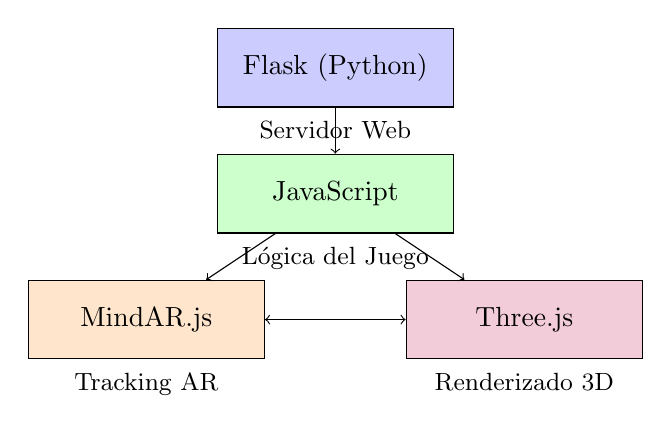
\begin{tikzpicture}[scale=0.8]
    % Backend
    \visible<1->{
    \node[draw, rectangle, minimum width=3cm, minimum height=1cm, fill=blue!20] (flask) at (0,4) {Flask (Python)};
    \node[below] at (0,3.3) {\small Servidor Web};
    }
    
    % Frontend Base
    \visible<2->{
    \node[draw, rectangle, minimum width=3cm, minimum height=1cm, fill=green!20] (js) at (0,2) {JavaScript};
    \node[below] at (0,1.3) {\small Lógica del Juego};
    }
    
    % AR Components
    \visible<3->{
    \node[draw, rectangle, minimum width=3cm, minimum height=1cm, fill=orange!20] (mindar) at (-3,0) {MindAR.js};
    \node[below] at (-3,-0.7) {\small Tracking AR};
    }
    
    \visible<4->{
    \node[draw, rectangle, minimum width=3cm, minimum height=1cm, fill=purple!20] (three) at (3,0) {Three.js};
    \node[below] at (3,-0.7) {\small Renderizado 3D};
    }
    
    % Connections
    \visible<5->{
    \draw[->] (flask) -- (js);
    \draw[->] (js) -- (mindar);
    \draw[->] (js) -- (three);
    \draw[<->] (mindar) -- (three);
    }
\end{tikzpicture}
\end{center}
\end{frame}

\begin{frame}
\frametitle{Arquitectura del Sistema con Three.js}
\begin{columns}
\column{0.5\textwidth}
\begin{itemize}
    \item<1-> \textbf{Capa de Renderizado 3D}:
    \begin{itemize}
        \item<2-> Three.js Scene Manager
        \item<3-> WebGL Renderer
        \item<4-> Camera Controls
    \end{itemize}
    \item<5-> \textbf{Integración AR}:
    \begin{itemize}
        \item<6-> MindAR para tracking
        \item<7-> Three.js para visualización
        \item<8-> Sincronización de matrices
    \end{itemize}
\end{itemize}

\column{0.5\textwidth}
\onslide<9->{
\begin{block}{Pipeline de Renderizado}
\begin{enumerate}
    \item Captura de video stream
    \item Detección de marcador AR
    \item Cálculo de pose 3D
    \item Three.js transforma matrices
    \item Renderizado WebGL
    \item Composición final
\end{enumerate}
\end{block}
}
\end{columns}
\end{frame}

% ============================================================================
% SECCIÓN 4: IMPLEMENTACIÓN CON THREE.JS
% ============================================================================
\section{Implementación con Three.js}

\begin{frame}
\frametitle{Three.js en SwipeMath AR}
\begin{itemize}
    \item<1-> \textbf{Motor de renderizado 3D}: Three.js maneja toda la visualización
    \item<2-> \textbf{Integración con MindAR}: Sincronización de cámara y tracking
    \item<3-> \textbf{Pipeline de renderizado}: Scene, Camera, Renderer
    \item<4-> \textbf{Gestión de recursos}: Modelos GLTF, texturas, materiales
\end{itemize}

\onslide<5->{
\begin{block}{¿Por qué Three.js?}
    \begin{itemize}
        \item WebGL simplificado
        \item Compatibilidad móvil/desktop
        \item Ecosistema robusto
        \item Rendimiento optimizado
    \end{itemize}
\end{block}
}
\end{frame}

\begin{frame}[fragile]
\frametitle{Configuración de la Escena Three.js}
\begin{lstlisting}[language=Java, basicstyle=\tiny]
// Inicializacion de Three.js con MindAR
const mindarThree = new MindARThree({
    container: arContainer,
    imageTargetSrc: '/static/assets/targets/targets.mind'
});

const {renderer, scene, camera} = mindarThree;

// Configuracion del renderer
renderer.setPixelRatio(window.devicePixelRatio);
renderer.setSize(window.innerWidth, window.innerHeight);
renderer.outputEncoding = THREE.sRGBEncoding;

// Iluminacion de la escena
const light = new THREE.HemisphereLight(0xffffff, 0xbbbbff, 1);
scene.add(light);

// Luz direccional para sombras
const directionalLight = new THREE.DirectionalLight(0xffffff, 0.8);
directionalLight.position.set(0, 10, 5);
scene.add(directionalLight);
\end{lstlisting}
\end{frame}

\begin{frame}[fragile]
\frametitle{Carga y Manipulación de Modelos 3D}
\begin{lstlisting}[language=Java, basicstyle=\tiny]
// Carga del modelo GLTF con Three.js
import {GLTFLoader} from 'three/examples/jsm/loaders/GLTFLoader.js';

async function loadStitchModel() {
    const loader = new GLTFLoader();
    const gltf = await loader.loadAsync(
        '/static/assets/models/stitch/scene.gltf'
    );
    
    // Configurar el modelo
    stitch = gltf.scene;
    stitch.scale.set(0.2, 0.2, 0.2);
    stitch.rotation.y = Math.PI;
    
    // Animar el modelo con Three.js
    mixer = new THREE.AnimationMixer(stitch);
    if (gltf.animations.length > 0) {
        const action = mixer.clipAction(gltf.animations[0]);
        action.play();
    }
    
    return stitch;
}
\end{lstlisting}
\end{frame}

\begin{frame}[fragile]
\frametitle{Sistema de Detección de Posición 3D}
\begin{lstlisting}[language=Java, basicstyle=\tiny]
// Raycasting para interaccion 3D
const raycaster = new THREE.Raycaster();
const mouse = new THREE.Vector2();

// Conversion de coordenadas AR a espacio 3D
function updateStitchPosition() {
    // Obtener posicion del marcador en el mundo
    const markerPosition = anchor.group.position;
    
    // Aplicar transformaciones Three.js
    stitch.position.copy(markerPosition);
    
    // Detectar lado para seleccion
    const worldPos = new THREE.Vector3();
    stitch.getWorldPosition(worldPos);
    
    // Proyectar a coordenadas de pantalla
    const screenPos = worldPos.project(camera);
    
    if (screenPos.x < -0.15) {
        highlightChoice('left');
    } else if (screenPos.x > 0.15) {
        highlightChoice('right');
    }
}
\end{lstlisting}
\end{frame}

\begin{frame}[fragile]
\frametitle{Renderizado y Animación con Three.js}
\begin{lstlisting}[language=Java, basicstyle=\tiny]
// Loop de renderizado principal
function animate() {
    requestAnimationFrame(animate);
    
    // Actualizar animaciones del modelo
    if (mixer) {
        const delta = clock.getDelta();
        mixer.update(delta);
    }
    
    // Rotacion suave del personaje
    if (stitch && gameActive) {
        stitch.rotation.y += 0.01;
        
        // Efecto de flotacion
        stitch.position.y = Math.sin(Date.now() * 0.001) * 0.05;
    }
    
    // Actualizar elementos UI en 3D
    updateOperationLabels();
    
    // Renderizar escena
    renderer.render(scene, camera);
}

// Iniciar loop de animacion
animate();
\end{lstlisting}
\end{frame}

\begin{frame}
\frametitle{Características Three.js Implementadas}
\begin{columns}
\column{0.5\textwidth}
\begin{itemize}
    \item<1-> \textbf{Geometrías y Materiales}:
    \begin{itemize}
        \item<2-> PlaneGeometry para UI
        \item<3-> MeshBasicMaterial
        \item<4-> TextureLoader
    \end{itemize}
    \item<5-> \textbf{Iluminación}:
    \begin{itemize}
        \item<6-> HemisphereLight
        \item<7-> DirectionalLight
        \item<8-> AmbientLight
    \end{itemize}
\end{itemize}

\column{0.5\textwidth}
\onslide<9->{
\begin{itemize}
    \item \textbf{Animación}:
    \begin{itemize}
        \item AnimationMixer
        \item Clock para timing
        \item RequestAnimationFrame
    \end{itemize}
    \item \textbf{Optimización}:
    \begin{itemize}
        \item Frustum culling
        \item LOD (Level of Detail)
        \item Texture compression
    \end{itemize}
\end{itemize}
}
\end{columns}
\end{frame}

% ============================================================================
% SECCIÓN 5: RESULTADOS Y DEMOSTRACIÓN
% ============================================================================
\section{Resultados y Demostración}

\begin{frame}
\frametitle{Estados del Juego}
\begin{columns}
\column{0.5\textwidth}
\begin{center}
\visible<1->{
\includegraphics[width=0.9\textwidth]{assets/game-center.jpeg}
% Juego en acción con Stitch
\vspace{0.2cm}
\textbf{Juego en Acción}
}
\end{center}

\column{0.5\textwidth}
\begin{center}
\visible<2->{
\includegraphics[width=0.9\textwidth]{assets/finish-game.jpeg}
% Pantalla de fin del juego
\vspace{0.2cm}
\textbf{Fin del Juego}
}
\end{center}
\end{columns}

\onslide<3->{
\begin{block}{Sistema de Retroalimentación}
\begin{itemize}
    \item Efectos de sonido diferenciados
    \item Animaciones visuales
    \item Actualización inmediata de puntuación
\end{itemize}
\end{block}
}
\end{frame}

\begin{frame}
\frametitle{Características Implementadas}
\begin{columns}
\column{0.6\textwidth}
\begin{itemize}
    \item<1-> \textbf{Escenario Único} (requisito PC5)
    \item<2-> \textbf{Realidad Aumentada} funcional
    \item<3-> \textbf{ODS 4 - Educación de Calidad}
    \item<4-> Sistema de dificultad progresiva
    \item<5-> Retroalimentación auditiva y visual
    \item<6-> Interfaz intuitiva para niños
\end{itemize}

\column{0.4\textwidth}
\onslide<7->{
\begin{block}{Métricas del Juego}
\begin{itemize}
    \item Tiempo promedio: 2-5 min
    \item Edad objetivo: 6-8 años
    \item Operaciones: +, -, ×, ÷
\end{itemize}
\end{block}
}
\end{columns}
\end{frame}

% ============================================================================
% SECCIÓN 6: CONCLUSIONES
% ============================================================================
\section{Conclusiones}

\begin{frame}
\frametitle{Logros Técnicos con Three.js}
\begin{itemize}
    \item<1-> $\checkmark$ Renderizado 3D fluido en navegador web
    \item<2-> $\checkmark$ Integración exitosa Three.js + MindAR
    \item<3-> $\checkmark$ Pipeline de gráficos optimizado para móviles
    \item<4-> $\checkmark$ Gestión eficiente de recursos 3D (GLTF)
    \item<5-> $\checkmark$ Animaciones y efectos visuales en tiempo real
\end{itemize}

\onslide<6->{
\begin{block}{Contribución a Computación Gráfica}
    Demostración práctica de cómo Three.js permite crear experiencias AR educativas complejas con rendimiento óptimo en la web
\end{block}
}
\end{frame}

\begin{frame}
\frametitle{Trabajo Futuro}
\begin{itemize}
    \item<1-> \textbf{Expansión de Contenido}:
    \begin{itemize}
        \item<2-> Más tipos de operaciones matemáticas
        \item<3-> Problemas de lógica y geometría
    \end{itemize}
    \item<4-> \textbf{Mejoras Técnicas}:
    \begin{itemize}
        \item<5-> Soporte multijugador
        \item<6-> Analytics de aprendizaje
        \item<7-> Más modelos 3D y animaciones
    \end{itemize}
    \item<8-> \textbf{Características Sociales}:
    \begin{itemize}
        \item<9-> Tabla de puntuaciones
        \item<10-> Modo competitivo
    \end{itemize}
\end{itemize}
\end{frame}

\begin{frame}
\frametitle{¡Gracias!}
\begin{center}
\Large
\textbf{SwipeMath AR}\\
\vspace{0.5cm}
\normalsize
Implementación de gráficos 3D con Three.js\\
para educación matemática en AR\\
\vspace{0.5cm}
\small
\textit{Demostrando el poder de Three.js para}\\
\textit{crear experiencias educativas inmersivas en la web}\\
\vspace{0.5cm}
\textit{Práctica Calificada 5 - Computación Gráfica}\\
\vspace{0.3cm}
\footnotesize
Repositorio: \url{https://github.com/thsergitox/pc5-grafica}
\end{center}
\end{frame}

\end{document}